\documentclass[english, a4paper, 12pt, twoside]{book}

% -------------- Setup, do not change these ---------------
\usepackage{textcomp}
\usepackage[T1]{fontenc, url}
\usepackage[utf8]{inputenc}
\usepackage{titlesec}
\setcounter{secnumdepth}{4}
\usepackage{multirow}
\usepackage{braket}


\usepackage{adjustbox}
\usepackage{graphicx}
\usepackage{wrapfig}
\usepackage{amsmath, amssymb, amsthm} % Mathematical packages
\usepackage{parskip} % Removing indenting in new paragraphs
\urlstyle{sf}
\usepackage{color}
\usepackage{subcaption}
\usepackage{appendix}
\usepackage{chngcntr} % needed for correct table numbering
\counterwithin{table}{section} % numbering of tables
\counterwithin{figure}{section} % numbering of figures
\numberwithin{equation}{section} % numbering of equations
\hyphenpenalty=100000 % preventing splitting of words
\sloppy
\raggedbottom
\usepackage{xparse,nameref}
\usepackage[bottom]{footmisc} % Fotnotes are fixed to bottom of page


% --------- You can edit from this point on --------


% ----- Appearance and language -----
\usepackage[english]{babel} % document language
\graphicspath{{./img/}} % path to images
\usepackage[margin=2.54cm]{geometry} % sets margins for the document
\usepackage{setspace}
\linespread{1} % line spread for the document
\usepackage{microtype}


% ----- Sections -----
\titleformat*{\section}{\LARGE\bfseries} % \section heading
\titleformat*{\subsection}{\Large\bfseries} % \subsection heading
\titleformat*{\subsubsection}{\large\bfseries} % \subsubsection heading
% next three lines creates the \paragraph command with correct heading
\titleformat{\paragraph}
{\normalfont\normalsize\bfseries}{\theparagraph}{1em}{}
\titlespacing*{\paragraph}
{0pt}{3.25ex plus 1ex minus .2ex}{1.5ex plus .2ex}


% ----- Figures and tables -----
\usepackage{fancyhdr}
\usepackage{subfiles}
\usepackage{array}
\usepackage[rightcaption]{sidecap}
\usepackage{wrapfig}
\usepackage{float}
\usepackage[labelfont=bf]{caption} % bold text for captions
\usepackage[para]{threeparttable} % fancy tables, check these before you use them
\usepackage{url}
\usepackage[table,xcdraw]{xcolor}
\usepackage{makecell}
\usepackage{hhline}
\usepackage{booktabs}

\usepackage[breaklinks=true,colorlinks=true,linkcolor=black,urlcolor=blue,citecolor=blue]{hyperref}
% ----- Sources -----


%\bibliographystyle{apa} % citation and reference list style
%\def\biblio{\clearpage\bibliographystyle{apa}\bibliography{References.bib}} % defines the \biblio command used for referencing in subfiles - DO NOT CHANGE


% ----- Header and footer -----
\pagestyle{fancy}
\fancyhead[RO,LE]{\thepage} % page number on right for odd pages and left for even pages in the header
\fancyhead[RE,LO]{\nouppercase{\rightmark}} % chapter name and number on the right for even pages and left for odd pages in the header
%\renewcommand{\headrulewidth}{0pt} % sets thickness of header line
\fancyfoot{} % removes page number on bottom of page


% ----- Header of the frontpage -----
\fancypagestyle{frontpage}{
	\fancyhf{}
	\renewcommand{\headrulewidth}{0pt}
	\renewcommand{\footrulewidth}{0pt}
	\vspace*{1\baselineskip}

	%\fancyhead[R]{Norwegian School of Economics
	%\linebreak       Bergen, Fall 2018\vspace*{5\baselineskip}}
	\fancyhead[C]{ \includegraphics[width=3.5in]{img/logo}}
}


% ----- Document starts here -----
\begin{document}

%\def\biblio{} % resets the biblio command, if not here a new reference list will be produced after every chapter
{\setstretch{1.5}

\begin{titlepage}

 \newgeometry{top=1 in, bottom=1 in, left=1 in, right= 1 in}

 \thispagestyle{frontpage}

 \begin{center}

   \vspace*{6\baselineskip}


   {\Huge \textbf{A single-ion-focused 393$\,$nm laser for photon generation and qubit control\\}}



       \vspace*{1,5\baselineskip}


   \vspace{1,5\baselineskip}

   \large{A master’s thesis submitted to the faculty of mathematics, computer science and physics, of the University of Innsbruck\\ in partial fulfillment of the requirements for the degree of\\\vspace{1,2\baselineskip}\textbf{Master of Science (MSc)} \\\vspace{1,2\baselineskip}carried out at the Institute of Experimental Physics under the supervision of}\\
   \large{o.Univ.-Prof.  Dr.  Rainer Blatt,}\\
   \large{Dr. Ben Lanyon}\\
    \vspace{1,2\baselineskip}
   \large{Presented by\\}
   \huge{\textbf{Marco Canteri}}\\
   \vfill
   \large{ }

 \end{center}

\end{titlepage}

}
\restoregeometry % restores the margins after frontpage
%\nocite{*} % uncomment if you want all sources to be printed in the reference list, including the ones which are not cited in the text

\pagenumbering{gobble} % suppress page numbering
\thispagestyle{plain} % suppress header
\clearpage\mbox{}\clearpage % add blank page

\pagenumbering{roman} % starting roman page numbering
\newpage

\section*{Abstract}
The purpose of this work is to build an optical system that enables single ion experiments in a linear Paul trap.
% Ions are separated typically by 4-6 $\mu$m, hence a laser must be focused more narrowly in order to control one single ion in a crystal.
In this thesis a focusing setup for a 393nm laser is designed, simulated, and ultimately built. The setup comprises of an acousto-optical deflector (AOD), for steering the beam in the microsecond timescale, and a set of lenses for expansion and control of the laser beam, which is focused in the trap by a custom objective. Our experiment traps $^{40}\text{Ca}^+$ ions, that can be used for quantum computing and as a node in a quantum network. The 393nm laser in calcium implements two operations: a phase shift qubit gate by driving the transition in the far detuned regime, and single photon generation via a cavity enhanced Raman process. We report two experiments that demonstrate these two operations. The first experiment applied the qubit gate to a single ion in a 4-ion string, the phase shift is measured with a Ramsey interferometer. In addition to demonstrate single qubit manipulation, this experiment also allows for a measure of the focus spot of the laser: 1.2-1.3 $\mu$m with an upper bound of the addressing error of $10^{-3}$. The second experiment generated single photons out of a single ion in a string opening up new possibilities for our quantum network node.
\newpage


\newpage
\tableofcontents


\newpage
\addtocontents{toc}{\protect\setcounter{tocdepth}{4}} % sets depth of toc to 4, 1.1.1.1
\pagenumbering{arabic} % Starting arabic page numbering
\setcounter{page}{1} % sets pagecounter to 1

\chapter{Introduction} % section/chapter name
The next natural step in technology advancement is represented by quantum technology, as it offers a radically new approach for computation, communication, simulation, and metrology \cite{quantumtech}. All of these fields can greatly flourish with the development of quantum computers and quantum networks. Classical computers are limited in solving some particular problems that scale exponentially, and therefore a new approach is needed. Quantum computing can exploit particular features of quantum mechanics that have no classical counterparts, this allows for a speed up for a certain class of problems such as factorizing numbers \cite{shor}, or searching in a database \cite{grover}. Moreover, simulating nature at its quantum level is a hard task for classical computer, while quantum computers are naturally prone to simulate quantum dynamics.\\
Quantum networks also bring new additional features, and several benefits to communication. The concept of a quantum internet is to have a quantum channel along side with the classical channel, enabling the transmission of quantum information \cite{Wehnereaam9288}. The task of building a quantum network is not trivial, as there are fundamental differences with a classical link. Although the medium can be the same, such as optical fiber, a quantum network must have additional abilities, such as distributing entanglement, or transmitting quantum states. However, once achieved, quantum networks have several applications: cryptographic wise they allow for more secure information transmission through Quantum Key Distribution \cite{qkd2}, secure identification \cite{secureident}, blind quantum computation \cite{blindcomputation} and more \cite{Wehnereaam9288}. Outside cryptography, quantum networks finds applications in metrology: entanglement can be exploited to improve clock synchronization \cite{quantumclocks},
and extend telescope's baseline  \cite{telescope}. Furthermore, quantum networks offer more efficient solutions to distributed system problems \cite{distributedcomputing}.\\
A set of criteria exists to assess the viability of a realistic implementation of quantum computers and quantum networks \cite{divincenzo}, several platforms have been proposed and implemented trying to satisfy these criteria. Ion trapping has already fulfilled all criteria experimentally \cite{trappedions} and it shows great potential for a possible large scale quantum computer. The idea is simple, qubits are encoded in the electronic state of single trapped ion in a Paul trap. Manipulation can be done with laser pulses \cite{ionquantumcomputer} and by placing a cavity, an ion trap gains a controllable network interface \cite{stuteinterface}.\\
However, still a lot of challenges needs to be addressed for a quantum computer to outperform a classical one. Due to the incredible delicate nature of qubits, they are subject to decoherence which harms the successfulness and computational power of quantum computers. Therefore, scaling the number of qubit has been proven to be a difficult engineeristic challenge. Several solutions are possible: the number of qubits can scale; the dimension of qubits can decrease; or qubits can be linked together. The last solution is the approach at the base of quantum networks. The idea is to link several quantum computers to create a cluster of nodes that can work jointly.\\
It is in this context that this thesis arises. Currently there is an ongoing project of building a three node quantum network between two buildings on the campus of the University of Innsbruck. The third node is located in IQOQI, where the thesis took place. Here an ion trap is used as node of the network and it is connected to the other traps via a 400m fiber link. A 393nm lasers is responsible for the generation of the transmitted photons via a cavity enhanced Raman process \cite{stuteinterface}. At the time of this thesis' start, the 393nm laser was shining on every ion in the trap. In this case, if an ion string were to be loaded, the light would couple to every ions and there would be no control over the single ion-photon pair. An addressing setup enables the generation of single photons from individual ions which opens up several possibilities in computer-network interfacing: multi-ion-multi-photon states can be generated, a quantum node gains quantum memory capabilities, and the possibility of multiplexing increases drastically the network bandwidth.

To overcome this limitation, an optical setup for the 393nm laser had to be built with the purpose of focusing the light to a single ion in a string. Moreover, the setup should have the ability to steer the beam on a fast scale $\sim\mu$s and focus it on a different ion. The goal of this thesis was to design and build such a system. The setup is per se not complex, but the design is critical, ions separation is typical in the order of $\mu$m, which means the light should be focused down to $1-2\,\mu$m, at the limits of the optical elements involved. The steering part is achieved with an acousto-optical deflector (AOD), such device deflects the laser light on microsecond timescales proportionally to the applied input frequency allowing to control remotely the beam pointing of the system.\\
Once completed, the system will allow to manipulate single ions in a string in two different ways differentiated by the laser regime. Hence, the final goal of the thesis is to perform two experiments that demonstrate the functionalities of the system:\vspace{-1em}\newline
\begin{center}{\large\textbf{\textsc{Single ion photon generation}}}\end{center}
\begin{wrapfigure}{l}{0.4\textwidth}
  \begin{center}
    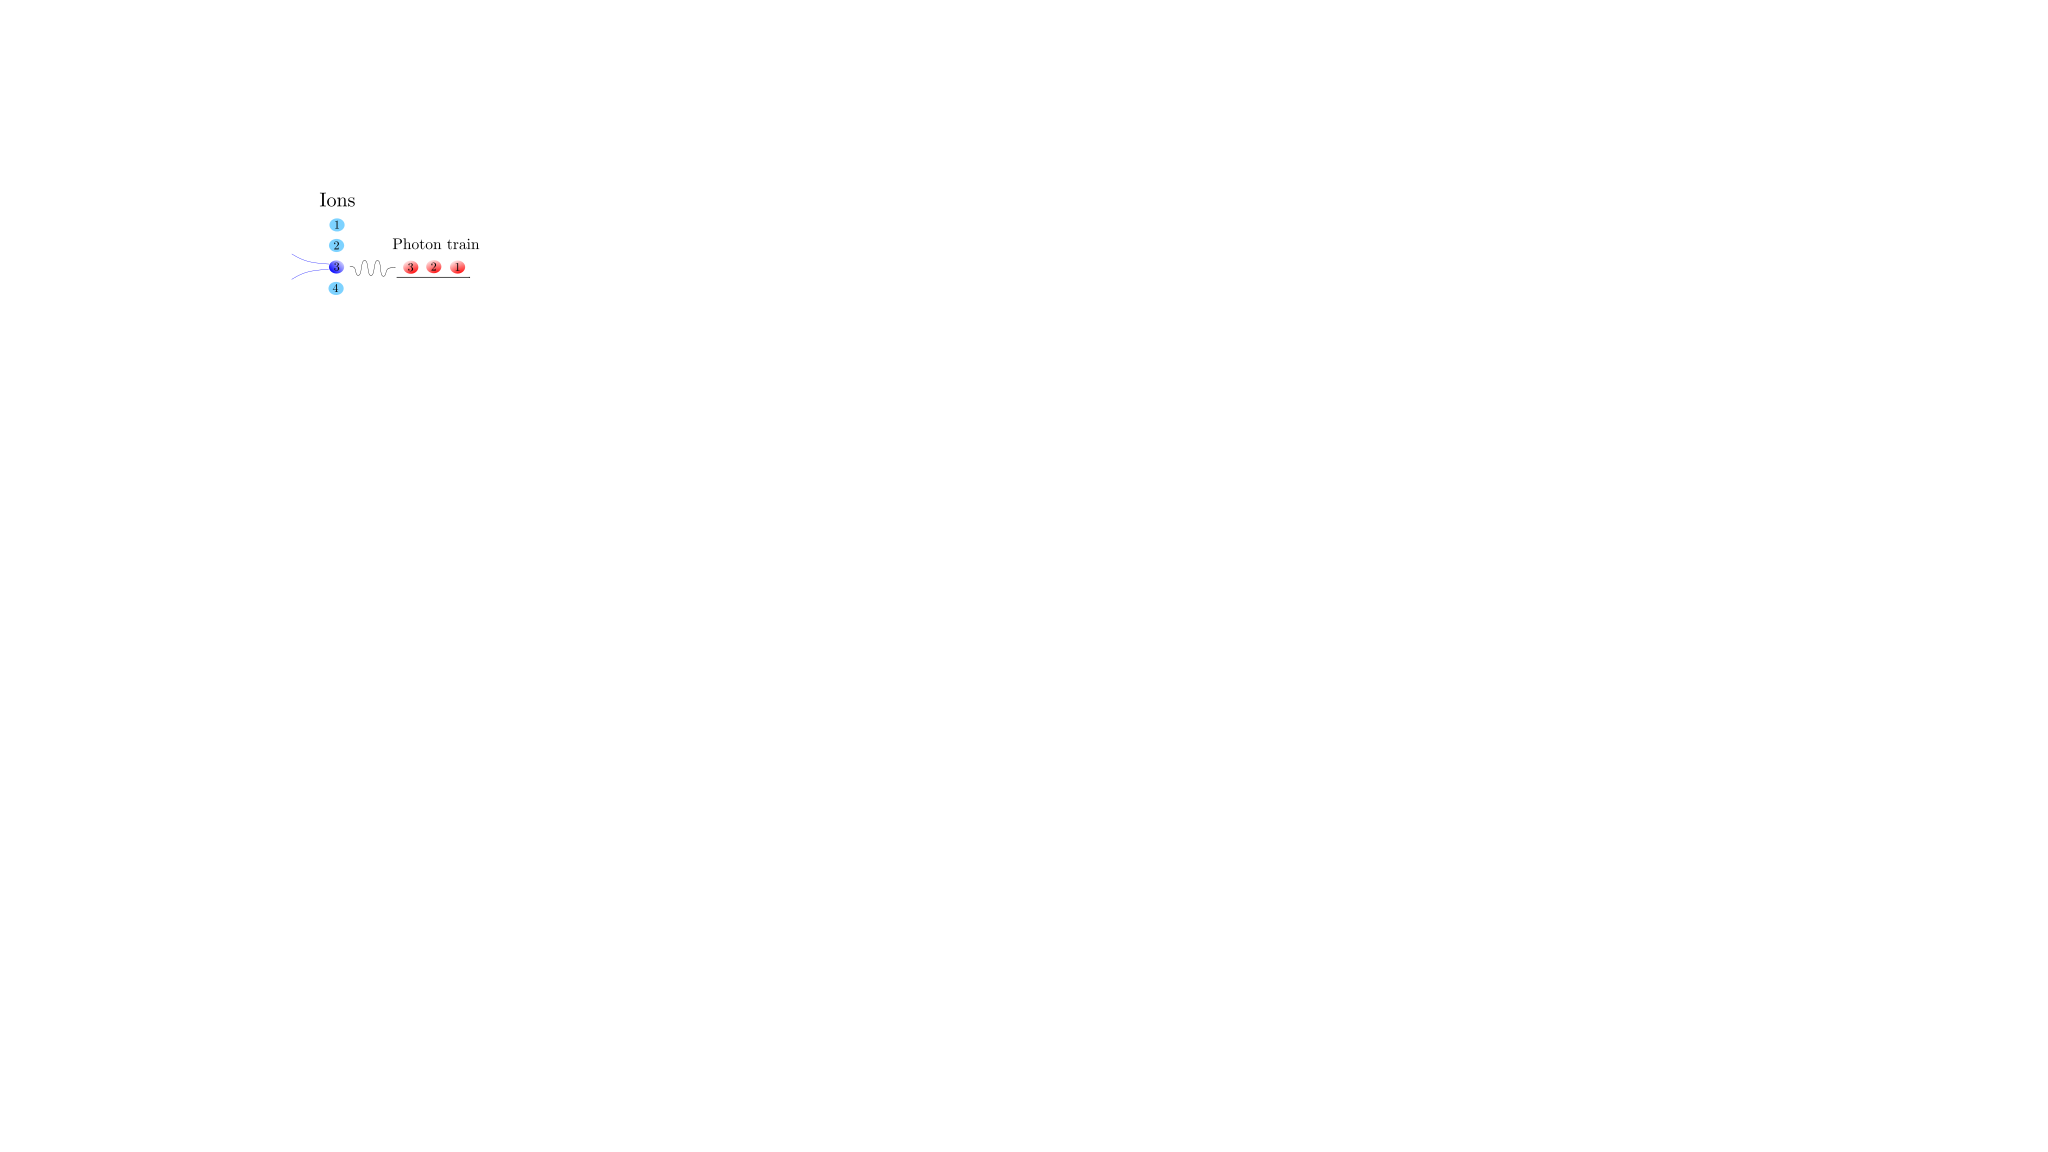
\includegraphics[width=0.4\textwidth]{photongeneration2}
  \end{center}
  %\caption{Schematic of photon generation}
\end{wrapfigure}

The first experiment is photon generation, a single laser pulse can trigger the generation of a single photon in a cavity via a Raman process \cite{stuteinterface}. The process requires the addressed ion to be coupled to the cavity electric field,
both the cavity and the laser pulse must be correctly detuned to suppress spontaneous scattering and maximize the probability of photon production. With the AOD the laser pulse is steered and aimed at different ions in $\mu$s time, thus enabling the creation of photon trains. This enriches the capabilities of the interface between the ion quantum computer and the photonic network channel, as outlined above.\vspace{-1em}\newline
\begin{center}{\large\textbf{\textsc{Single ion qubit manipulation}}}\end{center}
\begin{wrapfigure}{R}{0.4\textwidth}
  \begin{center}
    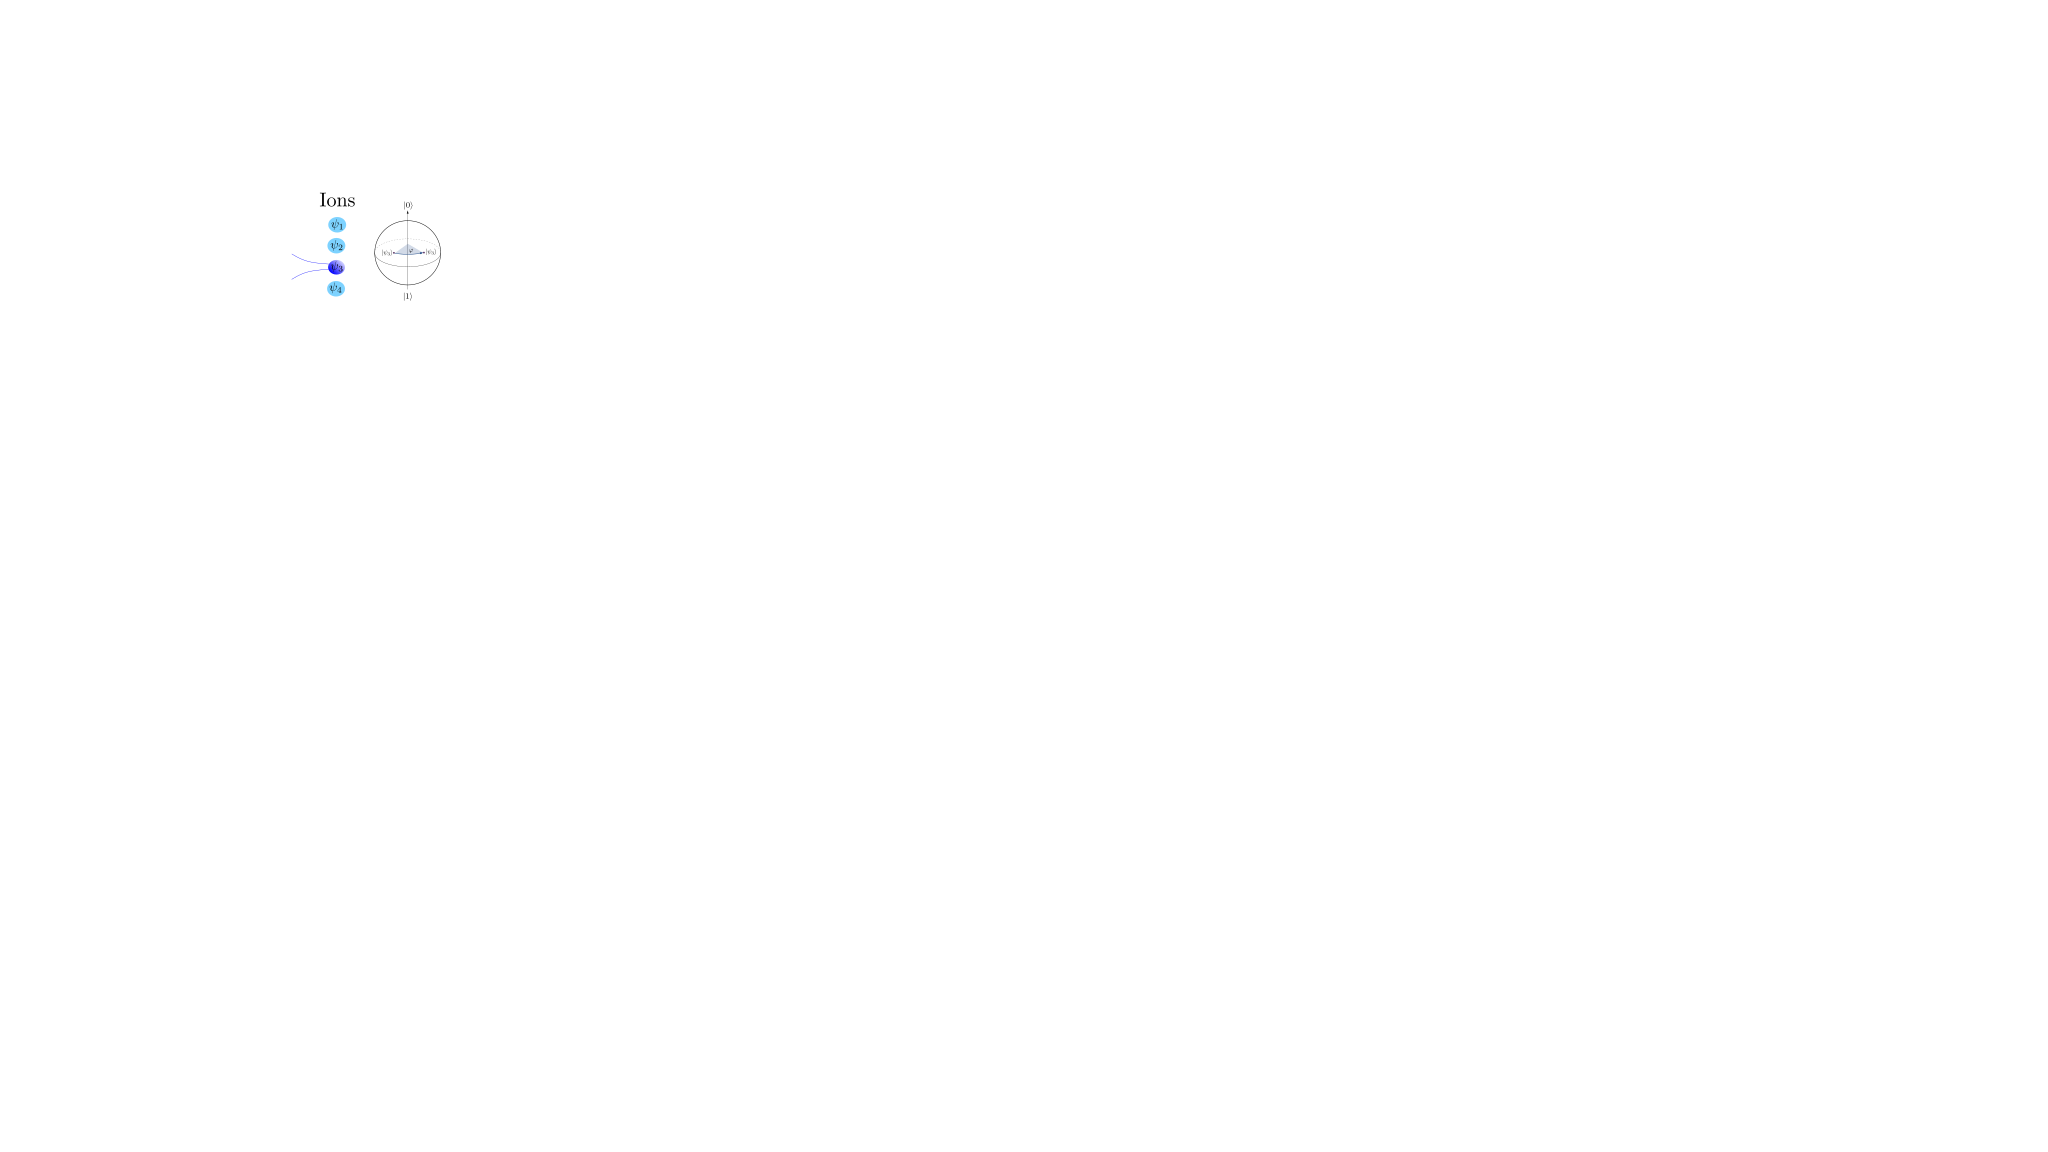
\includegraphics[width=0.4\textwidth]{qubitmanipulation2}
  \end{center}
  %\caption{Schematic of photon generation}
\end{wrapfigure}
The second experiment is qubit manipulation. A phase gate \cite{chuang} over a single qubit is implemented. In the off resonant regime, the laser induces AC Stark shift on the $\ket{0}$ state of the qubit, shifting the relative phase of the qubit state. In order to measure the AC Stark shift we want to perform Ramsey interferometry \cite{starkshift}, where between the two $\pi/2$ pulses a detuned Stark pulse is introduced. This pulse shift the relative phase of the qubit and therefore the amount of Stark shift can be inferred from the final qubit state. The gate is part of the universal set of quantum gates \cite{chuang}, and it is therefore a building block of a full implementation of a quantum computer.

This work is presented in the following way: Chapter 2 is devoted to the theoretical background necessary to understand the rest of the work. Here the foundations of quantum computing and networking are laid down, along with the basic concepts of ion trapping, and Gaussian beams; Chapter 3 presents the existing experimental setup, i.e. the already built and working blocks of the experiment where the setup designed in this thesis has been added; Chapter 4 is the core of the thesis, here the final design made with the software Zemax and simulations of different aspects of the project are introduced and presented;
Chapter 5 contains all the experimental results obtained. It is divided in two parts: First, the setup was built on a spare optical table, here we had the freedom to test different key properties of the performance of the system and decide whether or not it was satisfactory. After having the certainty that the system will work, the setup was transferred and aligned on the main experiment where limited access did not allow for easy performance testing. Here, different and more advanced experimental quantum optics methods had to be used to check if the system was working properly. The description and discussion of these results are in the second part of chapter 5. Lastly, in chapter 6 a conclusion with a summery and a future outlook is given.


% Theory chapter
\chapter{Theoretical framework}
Quantum computing is based on a general framework that does not depend on the physical platform. Here, important concept such as qubit, and quantum operations are described before showing how we can realize them, from a theoretical point of view, with trapped ions. The same goes with quantum networking, the concept and the realization can be treated separately and they will be described in this chapter. Furthermore, in this chapter we will take a look into Gaussian beams and their properties. Since that is the shape emitted by laser, it is important to understand their characteristic and how to manipulate them. Lastly Acousto-optical interactions are introduced and studied to give an idea of how AODs work and how they can be used to steer a laser beam.
\section{Quantum logic with trapped ions}
\subsection{Quantum computer and quantum gates}
The concepts of quantum computing are borrowed and extended from classical computational theory. In the classical case, information is represented in terms of binary digits, the so called bit, essentially mapping information to a base-2 number. Information processing is done with gates acting of those numbers. The idea of quantum computer is still to encode information in a binary form, but due to the nature of quantum mechanics, a quantum bit (in short qubit) gains new features that can be exploited to perform different kind of operations that in some cases are a speed up compared to the classical case.\\
A qubit is formally a normalized wave function that can be written as superposition of two orthogonal states indicated usually with $\ket{0}$ and $\ket{1}$:
\begin{equation}
\label{qubit}
\ket{\psi} = \alpha \ket{0} + \beta\ket{1},
\end{equation}
where $\alpha,\beta$ are probability amplitudes, two complex numbers that satisfy the relationship $|\alpha|^2+|\beta|^2 = 1$.
At first glance, the advantage of qubits seems obvious, while one classical bit can store only one bit of information, a qubit can be in any linear combination, i.e. $\alpha$ and $\beta$ can be chosen freely and any information can be represented. Although, the reality is different, due to rules of quantum mechanics, $\alpha$ and $\beta$ cannot be directly accessed, which means that we can get only a limited amount of information out of a qubit. The outcome of measuring a qubit will give the value 0 with a probability of $|\alpha|^2$ and 1 with a probability of $|\beta^2|$.  [..]

Qubits also have a geometrical representation that can be useful, equation \eqref{qubit} depends on 4 real numbers, however since $\psi$ is normalized, we can rewrite the expression as
\begin{equation}
\ket{\psi} = e^{i\gamma}\left(\cos\frac{\theta}{2}\ket{0} + e^{i\varphi}\sin\frac{\theta}{2}\ket{1}\right).
\end{equation}
the global phase factor $e^{i\gamma}$ can be left out, as it does not influence the measurement outcome. This leaves us with only two real number: $\theta$ and $\varphi$. A qubit is therefore representable with only these two numbers that we can chose to represent geometrically with normalized spherical coordinates. The so called Bloch sphere is depicted in figure \ref{blochsphere}, every point on its surface represents a different state of the qubit. Here qubit manipulation can be visualized as trajectories on the surface, which in some cases is very useful. The drawback of this representation is that it is limited to only one qubit, so it loses usefulness when dealing with multiple qubits.
\begin{figure}[H]
\centering
\includegraphics[width = .4\textwidth]{bloch_sphere}
\caption{The Bloch sphere. The states $\ket{0}$ and $\ket{1}$ are at the poles of the sphere, every other point of the surface represents a superpositions of these states. A quantum gate can be seen as trajectory on the surface mapping one state to another.}
\label{blochsphere}
\end{figure}

A more practical way of dealing with qubits is via matrices. We can assign to the states $\ket{0}$ and $\ket{1}$ the following:
\begin{equation}
\ket{0} = \begin{pmatrix}
 1 \\
 0
\end{pmatrix} \quad
\ket{1} = \begin{pmatrix}
 0 \\
 1
\end{pmatrix} \implies \ket{\psi} = \begin{pmatrix}
 \alpha \\
 \beta
\end{pmatrix}.
\end{equation}
In this representation, manipulations of qubits are easily calculated using $2\times2$ unitary matrices. These kind of operations are named \emph{quantum gates} and they are the building blocks of quantum computing. Every quantum algorithm can be written as a sequence of quantum gates and it is therefore important to understand them. For a single qubit any gate can be written as combination of two operations \cite{hempel}
\begin{equation}
U_z(\theta) =  \begin{pmatrix}
 e^{-i\frac{\theta}{2}} & 0 \\
 0 & e^{i\frac{\theta}{2}}
\end{pmatrix} \qquad U_\varphi(\theta) = \begin{pmatrix}
\cos\frac{\theta}{2} & -i e^{-i\varphi}\sin\frac{\theta}{2} \\
-ie^{i\theta}\sin\frac{\theta}{2} & \cos\frac{\theta}{2}
\end{pmatrix}.
\end{equation}
These two matrices can be seen as two different rotations in the Bloch sphere, $U_z$ is a rotation around the $z$ axis by the amount $\theta$, while $U_\varphi$ is a rotation on the $x-y$ plane around an axis tilted by $\varphi$. examples [H gate, phase gate]\\
\newline
As we have seen, a single qubit has already the advantage of superposition compared to classical case. When considering multiple qubits, we gain even more quantum mechanical features like entanglement. This phenomenon does not have a classical analogy and it is an extremely useful tools in quantum information.\\
In general a state with $N$ qubits is written as tensor product of the single qubit states $\psi_i$
\begin{equation}
\ket{\psi_N} = \ket{\psi_1}\otimes \ket{\psi_2}\otimes \cdots \ket{\psi_N} \equiv \ket{\psi_1\psi_2\dots \psi_N}.
\end{equation}
If we had to write out explicitly all the probability coefficients of $\psi_N$, we would need $2^N$ complex numbers. It is clear then why classical computer cannot keep up. $N$ bits can only give $N^2$ different combinations, while the Hilbert space of qubits is exponentially larger.\\
Now, let us consider only 2 qubits, a particular case would be
\begin{equation}
\ket{\psi} = \frac{1}{\sqrt{2}}\left(\ket{00} + \ket{11}\right).
\end{equation}
If a measurement is made on one of the two qubit and, for instance, the outcome is 0, the wave function collapses to the state $\ket{00}$, collapsing also the state of the other qubit, even if no operation has been directly performed on it. Next you measure the the second qubit and the outcome will be 0 with unitary probability. Viceversa, if the outcome if the first measurement was 1, the state collapses to $\ket{11}$ and the outcome of the second measurement is always 1. The two qubits are correlated, but this correlations is stronger than the classical one.\\
Gates that involve multiple qubits are written as $2^N\times 2^N$ unitary matrices, a famous example is the CNOT gate, [..]

It can be shown [] that the examples we saw here, H gate, phase gate, and CNOT gate form a universal set of quantum gates, i.e. a sequence of these gates approximate every other quantum gate.

\subsection{Ion qubits and laser-ion interactions}
Qubits can be encoded in any pair of orthogonal states. In the case of an ion it is possible to take two internal electronic states. The choices are multiple: an optical qubit is implemented in an optical transition, an hyperfine qubit is between two hyperfine states, and a Zeeman qubit can be realized with two magnetically separated levels. We will take the choice of an optical qubit, in this case lasers provide an easy way to manipulate the population of the two level and therefore to manipulate the state of the qubit, implementing quantum gates in an almost straightforward way. As long as the chosen levels are well separated, and the light is near resonant to the transition, it is possible to describe the system with the basic 2-level atom scheme interacting with classical light. \\
In this section, the theoretical model of a 2-level atom is presented together with a model of interactions between the laser and the ion. This represents a physical implementation of the concepts illustrated in the previous section.
\begin{figure}[H]
\centering
\includegraphics[width = .4\textwidth]{2levelatom}
\caption{2-level atom scheme, the ground and excited states are denoted as $\ket{g}$, and $\ket{e}$. $\omega_l$ is the laser frequency, which is detuned by $\Delta$ from the transition frequency $\omega_0$.}
\label{2levelatom}
\end{figure}

Consider the system in figure \ref{2levelatom}, the Hamiltonian of the atomic part can be written as:
\begin{equation}
H_a = \hbar\omega_0 \ket{e}\bra{e},
\end{equation}
where $\omega_0$ is the frequency difference between the ground and excited state, the energy of the ground state has also been set to 0. The Hamiltonian of the interaction between light and atom can be written as []
\begin{equation}
H_{int} = -d\cdot E
\end{equation}


- 2 level atom scheme\\
- Model of laser-ion interaction: rabi flops, AC stark shift
\section{Quantum networking with trapped ions}
\subsection{General introduction}
- Nodes, interface, link, protocols\\
- logic, memory, interface, Bell pairs, purification, multi-mode
- Distributed entanglement
\subsection{Cavity QED}
- Simple model atom in cavity: g,gamma, k
\section{Basics of ion trapping}
\subsection{Linear Paul trap}
- How a Paul trap works\\
- micromotion?
\subsection{Ion strings}
We have seen that the potential inside the trap can be described as an harmonic potential. It is then possible to calculate the ion separation between $N$ ion loaded in the trap. This will give us an idea of how narrowly the beam should be focused and will set an appropriate problem spatial scale.\\
We will consider only the $z$ direction where the ions are weakly confined and will form a string. The harmonic potential is then given by
\begin{equation}
V = \sum_{i=0}^N \frac{1}{2}M\omega^2z_i^2 + \sum_{i\neq j}^N\frac{Z^2e^2}{8\pi \epsilon_0}\frac{1}{|z_i-z_j|}
\end{equation}
The equilibrium position can be found at the minima of the potential, i.e. where the first derivative zeros
\begin{equation}
\frac{\partial V}{\partial z_i} = 0 \implies u_i - \sum_{j=1}^{i-1} \frac{1}{(u_i-u_j)^2} + \sum_{j= i+1}^{N} \frac{1}{(u_i-u_j)^2}= 0,
\end{equation}
where we defined the dimensionless quantity $u_i = z_i/l$ and $l^3 = \displaystyle\frac{Z^2 e^2 }{4\pi \epsilon_0 M\omega^2}$.
The last equations can be solved analytically only for 2 or 3 ions. In fact, for the case $N=2$ we simply get the system
\begin{equation}
\begin{cases}
  u_1 + \frac{1}{(u_1-u_2)^2} = 0\\
  u_2 - \frac{1}{(u_1-u_2)^2} = 0
  \end{cases} \quad \implies \quad u_1 = -u_2,\quad  u_1 = \left(\frac{1}{2}\right)^{2/3} \simeq 0.629
\end{equation}
For calcium-40 ions in a Paul trap with axial confinement of 1MHz, we have $l \simeq 4.45\times 10^{-6}\, \mu$m, which means that 2 ions are separated by $\simeq 5.6\, \mu$m. In the case of more ions the separation is lesser with the same confinement, but it is also possible to lower the axial frequency and increase the separation between the ions such that also in the case of several ions, the distance between them is still in the order of several $\mu$m. This size is accessible with current focusing optics and it is above the diffraction limit.\\
For more ions, a numerical approach has to be used, \cite{ion_spacing} reports values of $u_i$ up to $N=10$, and gives an empirical formula of the minimum separation
\begin{equation}
u_{min}(N) \simeq \frac{2.018}{N^{0.559}}
\end{equation}
\subsection{Doppler cooling and detection}
\section{Laser beam}
\subsection{Gaussian beams}
Lasers emit light in the shape of Gaussian beams, so it is import to understand what Gaussian beams are and their characteristics. In this chapter we will take a closer look into such beams and introduce important quantities to characterize a Gaussian beam. \\
From a theoretical point of view, Gaussiam beams are solution of the Helmholzt equation
\cite{saleh}
- Introduction to import quantities, like FWHM, focus, waist!
\subsection{Diffraction limit}
- To search whats limiting the diffraction, (lambda/2)
\subsection{Beam stearing via AOD's}
- How AODs work, simple Model\\
- Introduce diffraction efficiency, bandwidth


%Existing experimental setup chapter
% !TEX root = main.tex

\chapter{Existing experimental system}
The work developed in this thesis lies on top of an existing experiment. In this chapter we are going to describe the essential parts of the already existing setup on top of which the addressing system has been build. Calcium-40 ions are used in the experiment, the implementation of several techniques for
trapping and manipulating these ions are discussed. Furthermore, the addressing setup utilizes 393 nm light, the laser emitting this light was already installed and used, thus that setup is presented. The experiment can be controlled remotely via computers, an overview of how it is implemented and how it works is also given.

\section{Ion trap and key techniques}
\subsection{Calcium Ions}
\begin{figure}
\centering
\includegraphics[width = .6 \textwidth]{calciumscheme}
\caption{Level scheme of $^{40}\text{Ca}^+$ with main transitions highlighted. Blue transitions are dipole transitions suitable for cooling, imaging and photon detection. Red transitions are dipole forbidden, but accessible with electric quadrupole, they are used to encode qubits. Orange transition are usually repumped. In addition, the 854 nm transition is tuned in resonance with the cavity for photon generation purposes. From more and precise value see table \ref{transitiontable}}
\label{calciumscheme}
\end{figure}
In choosing the appropriate ion to trap, one looks first of all for simplicity, which means choosing an element with one single electron in the most outer orbital.
This fact limits the choice to the second group of the periodic table, many of these elements has been successfully trapped: beryllium \cite{beryllium}, barium \cite{barium}, strontium \cite{strontium}, and calcium \cite{calcium}.
The latter has been chosen for this experiment, as calcium has transitions easily accessible with commercial diode and titanium-sapphire lasers. The most abundand isotope of calcium is calcium-40, which is a common choice, but not the only one \cite{Tanaka2007}. Nevertheless, $^{40}\text{Ca}^+$ ions were our choice. In figure \ref{calciumscheme} the level scheme of the only electron in the outer shell is presented. A single ground state is present $\text{S}_{1/2}$ with no hyperfine structure as $^{40}\text{Ca}^+$ does not posses a nuclear spin. There are two short lived excited states ($\sim 7$ ns): $\text{P}_{1/2}$, and $\text{P}_{3/2}$ which are accessible with dipole transitions. These states have different decay channel, for $\text{P}_{1/2}$
the branching ratios are $6\%$ to $\text{D}_{3/2}$, and $94\%$ back to the ground state. For  $\text{P}_{3/2}$ there is a probability of $5.3\%$ to decay to   $\text{D}_{5/2}$, $0.6\%$ to go to  $\text{D}_{3/2}$ and $94\%$ to return to  $\text{S}_{1/2}$. Due to the short lifetimes of these two states, they are suitable for laser cooling and state detection, while the states $\text{D}_{3/2}$ and $\text{D}_{5/2}$
are metastable ($\sim 1$ s) since accessible with electric quadrupole transition. Since the lifetime of the D states are much greater than typical coherence time, they can encode a stable qubit and manipulated without worrying about dissipative process. Table \ref{transitiontable} summarizes details about the different transitions, and what they are used for. A more detailed description and implementation is discussed in the next section.

\begin{table}[H]
\centering
\begin{tabular}{c c c c c}
 \toprule
    {Transition} & {wavelength (nm)} & {Decay rate $\Gamma$} & Lifetime $\tau$ & {Main use} \\ \midrule
   $\text{S}_{1/2} \to \text{P}_{1/2}$ & 396.847 & $2\pi \times 20.8$ MHz & 7.7 ns &  Cooling and imaging \\
    $\text{S}_{1/2} \to \text{P}_{3/2}$  & 393.366 & $2\pi \times 21.4$ MHz & 7.4 ns & Photon generation\\ \midrule
   $\text{S}_{1/2} \to \text{D}_{3/2}$ & 732.389 & $2\pi \times 0.132$ Hz & 1.080 s & - \\
    $\text{S}_{1/2} \to \text{D}_{5/2}$  & 729.147 & $2\pi \times 0.136$ Hz & 1.045 s   & Qubit  \\\midrule
    $\text{P}_{1/2} \to \text{D}_{3/2}$  & 866.214 &  $2\pi \times 1.70$ MHz  &  94.3 ns  & Repumping \\
    $\text{P}_{3/2} \to \text{D}_{5/2}$  & 854.209 & $2\pi \times 1.34$ MHz & 101 ns  & Cavity photon  \\
    $\text{P}_{3/2} \to \text{D}_{3/2}$  & 849.802 & $2\pi \times 1.52$ MHz  & 902 ns   & Repumping \\ \bottomrule
\end{tabular}
\caption{Transitions in $^{40}\text{Ca}^+$ and current use in the experiment. Values are taken from \cite{ion_spacing,stute}}
\label{transitiontable}
\end{table}



\subsection{Trapping, cooling, and state readout}
\begin{figure}
\centering
\includegraphics[width = .7\textwidth]{phototrap}
\caption{Photo of the mounted trap, a pair of compensation electrodes and the mirrors of the cavity are also visible.}
\label{trapphoto}
\end{figure}
Our trap is a linear 3D RF Paul trap as depicted in figure (), the picture of the real trap is displayed in figure \ref{trapphoto}. The trap consists of 4 ortoghonal electrodes with blade shape for RF confinement in the radial direction. In the axial direction confinement is achieved with two tip electrodes that forms the endcaps. Everything is made in titanium, it is covered in gold and the trap itself is mounted vertically on a Shappire holder. The endcaps are 5 mm apart, and they are usually kept at a voltage in the order of 500-1000V, which means an axial frequency of $\omega_z \sim 2\pi \times 0.7-1$ MHz. The four blades are 0.8 mm from the center of the trap and driven with an RF of $\sim 24$ MHz. Due to the high power delivered to this blades ($\sim-4$ dBm), the RF signal has to be impedance matched with the trap, this is done with an helical resonator.
The trap also includes three pairs of compensations electrodes that can be used to compensate micromotion.
Loading of ions is done with an atomic oven, calcium is heated a directed towards the trap, in the trap the atoms undergo 2-stage photon ionization. The first laser 375 nm, excite one electron to a very high excited state, the second laser 422 nm, brings the electron to free space ionizing the atom. Such two stage process allows to filter for isotopes and ionize only $^{40}\text{Ca}$. Loading usually takes minutes or tens of minutes depending on the number of ions one wants to load. Once loaded, ions are laser cooled with 397 nm light on the transition $\text{S}_{1/2} \to \text{P}_{1/2}$ detuned at $-\Gamma/2$. An additional repumper on the transition $\text{P}_{3/2} \to \text{D}_{5/2}$ is also used to avoid for the electron being stuck in the $\text{D}_{5/2}$ state. For typical experiment a stage of doppler cooling is always included, this lasts from 1 millisecond up to tens of milliseconds.\\
With the same Doppler cooling light, imaging can also be done. The light shines on the ions exciting the transition $\text{S}_{1/2} \to \text{P}_{1/2}$ driving the electron to the excited states which then decay spontaneously emitting a photons. Photon are collected with a custom objective with NA of $\sim 0.3$, which means an efficiency of 2.5 \% over the solid angle $4\pi$. The objective focuses the collected photons 1.5 meters away where a CCD camera (Andor iXon Ultra 897) is placed. The geometrical path of the imaging is displayed in figure (), the same objective is also used for the addressing setup built within this thesis. Therefore, the imaging optical path must be partially shared with the newly built addressing. In depth overview of objective is therefore given in section ().\\
State read out is possible with this kind of imaging. Consider a qubit encoded in the states
$\text{S}_{1/2} \to \text{D}_{5/2}$, if the imaging laser is switched on, the electron will be projected either to the $\text{S}_{1/2}$ level or in the $\text{D}_{5/2} $. In the first case, photons are scattered from the ion and collected on the camera, in the second case the electron is shelved and will not scatter any photon. Hence, the two cases are distinguishable by counting statistics. An histogram can be constructed  with the number of photon measured, and a properly set threshold differentiates between bright and dark states. Typical detection times are in the order of milliseconds.



\subsection{Photon generations}
- Cavity enhanced Raman transition
\section{393nm laser}
\section{Experiment control}


%Design and simulation
% !TEX root = main.tex
\chapter{Design and simulation of the addressing setup}
The purpose of this thesis work was to design and build the addressing setup for the already existing experiment. In this chapter we discuss the design and the implementation of such setup. The design is a crucial part of the work, there are several requirements that have to be met in order to achieve the proper needed functionality. In the first section, the requirements are presented together with an overview of the design idea. In the setup an objective was already present, ad the choice of an AOD was already made. Hence, we discuss this components as given. The rest of the setup was simulated with the software Zemax, which was used to find the optimal optical components and their placement.
\section{Addressing system overview and requirements}
Addressing systems have already been developed and employed in experiments successfully. Different techniques are available: the main idea is to focus a laser beam tighter than ion-ion separation and steer it. In  Innsbruck calcium ions have been addressed in this way, where the steering was achieved with an AOD \cite{addressing}; Beam has also been steered with micro-electromechanical systems (MEMS) mirrors \cite{addressing3}. Another idea is to send a normal beam illuminating all the ions, but hiding those who are not addressed. This was done with Ytterbium atoms where by means of a inhomogeneous magnetic field the transition frequencies were shifted shielding selected ions \cite{addressing2}. \\
Our choice was to implement the already successful idea of Innsbruck with an AOD and improve it. The advantage of AODs is to have a fast switching time in the order of $\mu$s, that is used for fast switching between ions. A problem with the implementation of \cite{addressing} is however the fact that the AOD is placed right before the beam expander, this limits the addressing range, as the beam is likely to clip when it is steered on the edge of the AOD's bandwidth. This is the main problem that the new designed system, here implemented, wanted to address: exploiting the full capabilities of the AOD while maintaining a very tight focus.
Therefore, there are mainly two aspects to keep in mind, the focus spot and the addressing range.\\
The addressing setup should be able to address single ions in a string in order to generate single photons out of single ions via the already discussed Raman process. Ion separations, in the case of $^{40}\text{Ca}^+$, has been derived in section \ref{ionstrings}, for a trap frequency of 1 MHz is 5.6 $\mu$m. The setup must therefore be able to focus tightly a laser beam down to 1-2 $\mu$m. As seen in section \ref{sec_diffraction}, a tighter focus can obtained with a shorter wavelength, a bigger lens, or with shorter focal length. The focusing lens, a.k.a the objective, is shared with the imaging setup, and thus it is given, the focal length is therefore a constant in the problem. The wavelength is also a constant, as the Raman process happens only at 393 nm. This gives only one possibility left to tighten the focus, i.e. by making the beam as broad as possible at the objective input surface. Beam expansion can be achieved with a Galilean telescope, it take two lenses to form such Telescope, a concave Lenses to diverge a collimated beam and a convex lens to collimate the diverging beam. The combinations of these two lenses takes a collimated beam and expands it to another collimated beam. This expansion part is one of the two essential part of the addressing setup. The other part is related to addressing range. Not only, we want to focus the beam to a single ion, but we want to move the beam as well, such that it focuses on a different ion. Therefore, there is a requirement also on the range that can be addressed. This depends on the number of ions and their spacing, a good aim is to address tens of ions, this requires the ability to move the focus in one direction by 150-200 $\mu$m. Beam steering is possible with the use of an AOD, the detailed working principle of this device has been discussed in section \ref{theory_AOD}. Basically the angle of the output beam of the AOD changes as the driving frequency changes. However, the AOD must be placed far behind the objective to leave space for the beam expander, this implies a need to control and redirect the angle of the AOD's output beam to send it to the beam expander and later in the objective without any clipping. This task is accomplished with a pair of converging lenses, they refocus the collimated beam into the beam expander, beam then becomes wider, reaches the objective and it is focused on the ion. It is important to get the right lenses at the right distances, the objective has 5 different lenses inside and it works slightly differently from a normal lens. For instance, it does not focuses collimated blue light, but red. This means that the beam expander should not collimate completely the beam but rather expand it and leave it diverging, so that the objective can focus it at the right position.\\
The setup displayed in figure \ref{addressingsetup} also contains polarization optics. As discussed in section \ref{sec:ramanprocess}, Zeeman transitions are polarization sensitive, thus polarization control is required. The AOD is polarization sensitive, which means it requires a certain input polarization and outputs another particular polarization, that is the reason why half wave plate are before and after, and additional quarter wave plate is inserted before the objective to obtain circular polarized light. This placements means having a non standard plate, but if placed before in the optical path, the mirror and the beam splitter could alter the polarization. The choice of using a beam splitter is also peculiar, to separate light at different wavelength it is common choice to use a dichroic mirror, however the light in the imaging path is 397 nm, very close to the 393 nm light of the addressing setup. This would have meant using a very narrow dichroic, the alternative was to use a 90:10 beam splitter, where 90 \% of the light is transmitted and only 10 \%of the light is reflected. The addressing therefore loses 90 \% of the power on this splitter, but that is not a problem, since it is always possible to get more light out of the laser. Furthermore, this light is focused so tightly that even a small amount of light can excite the ions. On the other end, it is not really possible to get more scattered light from the ions, so 397 nm light and the imaging setup must be as efficient as possible, with 10 \% of losses, ions are still visible on the camera and on the PMT.

\begin{figure}
\centering
\includegraphics[width=\textwidth]{img/setup}
\caption{Setup scheme}
\label{addressingsetup}
\end{figure}

\section{Objective and AOD}
\label{sec:obj}
The objective used to focus the light was already present in the system and had to be taken as it is. It is a custom objective by Sill optics placed outside vacuum, the section is in figure \ref{objsection}. It contains 5 lenses inside a mechanical housing, the aperture is about 47 mm large in diameter.
This objective has different purposes, it was designed keeping in mind: imaging of ions, addressing with red light and addressing of blue light. The objective has to perform all three of this jobs fairly well, which means it has light transmission >90 \%, every lenses is AR coated, numerical aperture of NA = 0.3. Moreover, it is telecentric, which means that the focus spot should move perpendicularly to the optical axis if the beam is steered. Lastly it was also designed to take into consideration the fact that it is placed out of vacuum, the light after the objective has to go through a 6 mm fused silica viewport before entering the vacuum and after further 40 mm encounters the ions. The focal length of the objective is 54.07 mm at 729nm. The objective is also mounted on a 3 dimensional translational stage to allow for imaging and addressing calibration.
\begin{figure}[H]
     \centering
     \begin{subfigure}[b]{0.4\textwidth}
         \centering
         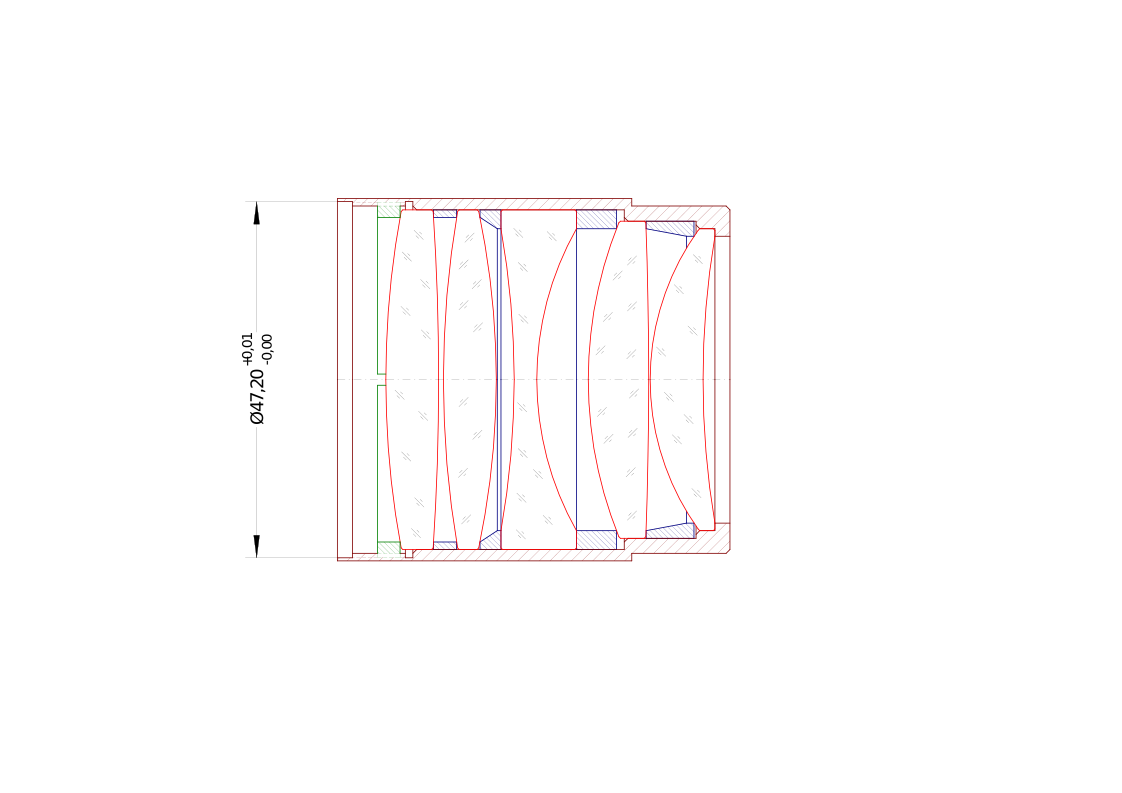
\includegraphics[width = \textwidth]{obj}
          \caption{Section of the custom objective, red parts are the lenses, while the rest is the housing.}
         \label{objsection}
     \end{subfigure}
     \hfill
     \begin{subfigure}[b]{0.55\textwidth}
         \centering
         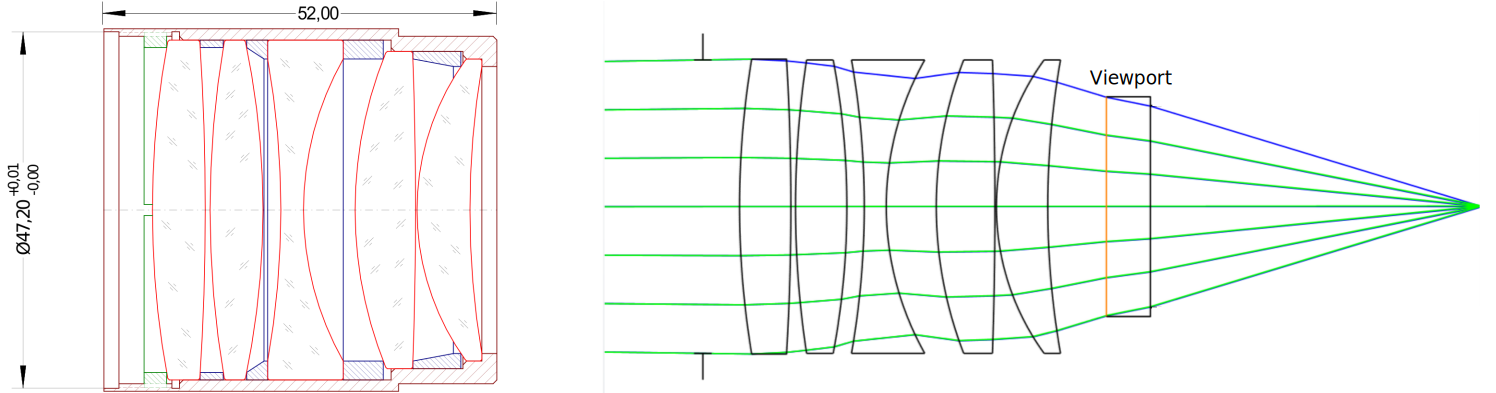
\includegraphics[width=\textwidth]{zeemaxobj}
         \vspace{1em}
         \caption{Zemax simulation of the objective. On the right, viewport and the vacuum chamber are also present.}
         %\label{fig:three sin x}

     \end{subfigure}
        \caption{}
      %  \label{fig:three graphs}
\end{figure}
The AOD is from Gooch \& Housego, model 4120-3. It has a specified central frequency of 120 MHz, with 50 MHz, bandwidth, so the driving frequency ranges from 95 to 145 MHz with a maximum RF power of 0.3 W. Therefore, the angle of deflection should be $\pm 0.86^{\circ}$ (:|).  In this bandwidth the diffraction efficiency should remain above 75 \% and have an average of 83 \%. Further light is lost as much as 3\% of due to insertion losses. The active aperture measures $3\times 3$ mm, and the polarization has to be horizontal when entering the AOD, while it gets rotated during diffraction, as the specified output polarization is vertical.

\section{Design simulation}
The setup in figure \ref{addressingsetup} has been simulated with the software Zemax. The simulation had the purpose of assessing the performance of the setup, i.e. checking the viability of the setup and see if it meets all requirements. It was also used to find the best lenses for building the setup and the best placement. Not everything was simulated, bu only the essential parts. This includes the four lenses, the objective, the viewport and the vacuum chamber. As there is no option to simulate an AOD, it was not taken in consideration, instead the simulation started at the output of the AOD as described below. Mirrors and beam splitters also do not alter drastically the optical path and therefore there was no need to simulate them.



\begin{figure}[H]
\centering
\includegraphics[width=\textwidth]{img/Plosses}
\caption{Losses on the compensation electrodes vs beam waist}
\end{figure}
\begin{figure}[H]
\centering
\includegraphics[width=\textwidth]{img/clipping}
\caption{Clipping on compensation electrodes}
\end{figure}

\section{Physical implementation}
- test setup
- picture
- alignment process



%Measurement results
% !TEX root = main.tex

\chapter{Experimental results}
\label{ch:results}
This chapter collects the key experimental results obtained during my master's work:
\begin{itemize}
\item Section \ref{sec:resultaod} contains the characterization of the AOD.
\item In Section \ref{sec:fullsetup} the characterization of the test setup is presented. Polarization, stability, and focus spot have been checked. In particular, two methods have been used to measure a $\mu$m focus spot: razor blade scans, and small pixel size camera.
\item In Section \ref{sec:finalsetup} the results from experiments with trapped ions are presented. First, single-qubit manipulation via Ramsey interferometry, which also allowed for a check of addressing performance. Second, a cQED experiment where single photons were generated from a single ion in a string, via a cavity-mediated Raman process (Section \ref{sec:ramanprocess}).
\end{itemize}
\section{AOD}
\label{sec:resultaod}
The two main parameters we are interested in are the diffraction efficiency and the response time. The response time is the For the diffraction efficiency we measured the total output power of the light $P_{tot}$ and then the power of the first diffracted order $P_{1}$. Diffraction efficiency is defined as the ratio between the two
\begin{equation}
\label{eq:de}
\text{DE} = \frac{P_1}{P_{tot}}.
\end{equation}
Before measuring the diffraction, the optimal RF power to drive the AOD has been found by maximizing the power of the first diffracted order with the AOD set at its central frequency. Power measurements of the light were done with a Thorlabs PM100D, and the AOD was driven with an amplifier and an RF signal generator. The highest efficiency at the central frequency was found for an RF power of 0.11 W, and for the rest of the measurements it was kept at that value. Furthermore, to optimize the linear input polarization, a PBS followed by a half-waveplate were placed before the AOD, the waveplate was rotated to maximize the power of the diffracted light. In Figure \ref{DE} a plot of the measured diffraction efficiency as a function of the RF frequency is displayed. Within a bandwidth of 50 MHz from 105 MHz to 155 MHz, we can see that more than 70 \% of the light is in the first diffracted order as expected from the datasheet (Appendix \ref{sec:aoddata}), even though the bandwidth looks shifted with respected to the nominal central frequency of 120 MHz.\\
The response time is the time it takes for the light to move to the new position corresponding to a RF frequency change. In order to perform this measurement, a voltage controlled oscillator (VCO) was used to generate the RF signal. The VCO was supplied a square wave that alternated between two voltages corresponding to two different frequencies $\sim 96$ and $\sim 127$ MHz. The laser light diffracted into the -1 order was measured with a photodiode. The photodiode was aligned with the light at one particular frequency, such that when the light moves, the beam would not hit the diode and the signal generated changes. In Figure \ref{response}, the signal of the photodiode, together with the supplied VCO signal are plotted. Response time is $\sim 8\,\mu$s, with $3\,\mu$s delay and $5\,\mu$s rise time. From the beam diameter (2.14 mm, $1/e^2$ of intensity) and the acoustic velocity in the crystal (0.65 mm/$\mu$s, Appendix \ref{sec:aoddata}) we expect $4.9$ $\mu$s rise time, while the delay indicates that the distance between the piezo and the edge of the beam is 1.95 mm.

\begin{figure}
\centering
\includegraphics[width = .95\textwidth]{DE2}
\caption{Measurement of the diffraction efficiency of the AOD as a function of the RF driving frequency (Equation \eqref{eq:de}). Blu stars indicate the measured points. Red points indicate the expected frequencies associated with addressing 4 ions for an axial COM frequency of 780 kHz (the conditions for the experiment presented in Section \ref{sec:singlequbitmanipulation}), the theoretical separations are 5.15 $\mu$m for the two outer ions, and 4.77 $\mu$m for the inner ions.}
\label{DE}
\end{figure}

\begin{figure}
\centering
\includegraphics[width = .95\textwidth]{response}
\caption{Response time of the AOD, plotted are the photodiode signal in blue on the left $y$ axis, and the VCO voltage is in red on the right axis. The voltage of the VCO determines the frequency of the RF sent to the AOD. The change here corresponds to a frequency shift of $\sim$31 MHz between $\sim 96$ and $\sim 127$ MHz. At the highest voltage, the photodiode measures the -1st diffracted light.}
\label{response}
\end{figure}

\section{Full test setup characterization}
\label{sec:fullsetup}
The test setup was built on an optical table with a spare objective since the one installed in the vacuum chamber was already in use for ion imaging. The layout of the system in Figure \ref{addressingsetup} was replicated.

\subsection{Waist: Knife-Edge method}
\label{sec:knifeedge}
\begin{figure}[H]
\centering
\includegraphics[scale = 1.1]{razorsetup}
\caption{Scheme of the razor scan. A translation stage allows for moving the blade in the direction x, perpendicular to the beam, and z, along the beam.}
\label{razorscan}
\end{figure}
Measuring a micrometer scale waist is not an easy task, the first method applied consisted of mounting a razor blade on a translational stage. The setup used is showed in Figure \ref{razorscan}, after the objective the blade is present, and since the beam is quickly diverging after the focus, a lens is used to refocus the light into a photodiode. The stage is moved in the $x$ direction cutting the beam perpendicularly such that the blade is scanning the beam profile. A filter was inserted in order to not saturate the photodiode.
In the $z$ direction the stage was controlled with a manual screw with resolution of $1\,\mu$m. While in the $x$ direction, the stage had to be moved with sub-micrometer precision, so instead there was a piezo actuator controlled by custom software. The same software also controlled a multimeter that measured the voltage of the photodiode. To get the profile $W(z)$ (equation \eqref{waistprofile}) of the beam, the measurement procedure was as follows
\begin{itemize}
\item Position blade at desired $z$ coordinate
\item Scan beam in $x$ direction with blade
\item Shift $z$ direction
\end{itemize}
The procedure is repeated for sufficient values of $z$ to scan at least a few Raylegh ranges. The beam width can be calculated from the scans by fitting the data with equation (2) of \cite{knifeedge}. In Figure \ref{examplerazorscan} we report an example of a scan that gave a minimal waist. The errorbars come from statistical average, every data point is a mean over 5 measurements, and the error is the standard deviation. The fit in this case gave a width $W$ (beam width $1/e^2$) of $3.47\pm 0.06\,\mu$m, the smallest width obtained with this method, but significantly broader than the 1 $\mu$m simulated waist. Furthermore, the profile $W(z)$ was not symmetric and could not be fitted with equation \eqref{waistprofile}. A possible explanation is that with this typically commercially-available razor blade, the accuracy is limited by the positioner and the blade roughness. The latter was not known at the few micrometer scale of the beam waist. In comparison, authors of \cite{Cannon:86} have used, instead of a common razor blade, a glass substrate etched with an effective knife-edge features with which they were able to measure a 1 $\mu$m waist.
\begin{figure}
\centering
\includegraphics[width=1\textwidth]{img/razorscan}
\caption{Razor scan at the waist of the beam $z=0$}
\label{examplerazorscan}
\end{figure}


\subsection{Waist: Camera}
\label{waistcamera}
Since the Knife-Edge method did not prove that we had achieved our desired waist, a  more direct approach has been subsequently adopted. We measured directly the beam with a camera from IDS model UI-1490LE-M-GL. This camera has a pixel size of 1.67 $\mu$m with no spacing between pixels. It should therefore be suitable to measure a focus spot with a $\mu$m precision. A 1 $\mu$m focus should hit one single pixel, and if aligned between two pixels, a Gaussian profile could also be fitted.
In addition, unlike the Knife-Edge technique, a camera provides 2-dimensional information about the beam shape and can be exploited to look for aberrations in the system. The setup is almost the same as Figure \ref{razorscan}, but the camera now replaces the razor blade, and there is no need for scanning in the $x$ direction, as the $z$ is enough to reconstruct the profile $W(z)$. An additional filter was used to optimize the light reaching the camera in order to not saturate it.
% \begin{figure}
%      \centering
%      \begin{subfigure}[b]{0.67\textwidth}
%          \centering
%          \includegraphics[width = \textwidth]{camera}
%           \caption{Fitted data from the camera. In red color, the normalized pixel value is displayed, while the blue curve is a fitted 2D Gaussian. On the axis there is the pixel number}
%      \end{subfigure}
%      \hfill
%      \begin{subfigure}[b]{0.3\textwidth}
%          \centering
%          \includegraphics[width=\textwidth]{cameraoriginal}
%         \vspace{5em}
%          \caption{Original photo from the camera.}
%          %\label{fig:three sin x}
%
%      \end{subfigure}
%         \caption{}
%        \label{fig:camera}
% \end{figure}
For every desired $z$ displacement, a photo with the camera is taken, post processed, and then the camera is displaced to the new $z$ coordinate. Post processing is done by fitting the pixel values with a 2-dimensional Gaussian
\begin{equation}
P = A \exp\left\{-\frac{(x-x_0)^2}{2\sigma_x^2}\right\} \exp\left\{-\frac{(y-y_0)^2}{2\sigma_y^2} \right\}.
\end{equation}
The fit parameters are $A,x_0,y_0,\sigma_x,$ and $\sigma_y$. From the standard deviations $\sigma_x$ and $\sigma_y$ the beam width in the $x$ and $y$ direction at position $z$: $W_x(z),W_y(z)$ can be determined as $W_x(z) = 2\cdot 1.67\cdot \sigma_x$ and respectively $W_y(z) = 2\cdot 1.67\cdot \sigma_y$, where $1.67\,\mu$m is the pixel size (see caption of Figure \ref{gauss}). The full profiles $W_x(z)$ and $W_{y}(z)$ can be found in Figure \ref{cameraprofile}. Here anomalies can be noticed. The profile is asymmetric and does not follow equation \ref{waistprofile}, nonetheless a width $<2.5\,\mu$m has been measured. We decided to install the system and measure more accurately the waist with a single ion.
\begin{figure}
\centering
\includegraphics[width=1\textwidth]{cameraprofile_inset}
\caption{Profile of the Gaussian beam along $z$ measured with the IDS camera. Errorbars are estimated from fit. In the inset an example of raw data and Gaussian fit. In red color, the normalized pixel value is displayed, while the blue curve is a fitted 2D Gaussian. On the axis there is the pixel number.}
\label{cameraprofile}
\end{figure}

\subsection{Polarization}
\label{sec:polarization}
As discussed in the design Section \ref{sec:addressing} and in the Raman process \ref{sec:ramanprocess}, polarization is an important component as atomic transitions are polarization sensitive, thus the polarization capabilities of the system had to be tested. The goal is to allow for the generation of vertical, horizontal, left circular, and right circular polarization at the ion position and test how well they are achieved. Polarization can be changed with two plates: a half wave plate after the AOD, and a quarter wave plate right before the objective, see Figure \ref{addressingsetup}. In order to characterize the polarization at various points in the optical path of the addressing setup, the three Stokes parameters $S_i$ \cite{stokes} were measured with a polarimeter from Sc\"after + Kirchhoff series SK010PA.\\
Stokes parameters quantify the type of polarization of an electric field. Linear polarized light has Stokes parameters $S_2,S_3 = 0$, while $S_1 = \pm 1$ for horizontal and vertical polarization respectively. Circular polarized light has $S_1, S_2 = 0$ and $S_3=\pm 1$ for right hand and left hand circular polarization respectively.\\
The first step was to characterize the polarization after the waveplate after the AOD ($\lambda/2$, WP B, Figure \ref{addressingsetup}), the main result from this characterization is that horizontal polarization can be achieved immediately after WP B with an angle of $267.2\pm 0.1 ^{\circ}$, and vertical is achieved with an angle of $312.5\pm0.1^{\circ}$ obtained from fitting a sine on the first Stokes parameter. From the same fit, the semiperiod of the polarization is $45.3\pm 0.6^\circ$ consistent with the $45^\circ$ expected for a half waveplate.\\
Afterwards, we measured the polarization after the objective at the focus spot where the ions ideally sit. For this measurement we set the $\lambda/2$ WP B first at $267.2^\circ$, and then at $312.5\pm0.1^{\circ}$, for both numbers we measured the three Stokes parameters as a function of the $\lambda/4$ angle. Results are summarized in table \ref{polarizationstable}, in appendix \ref{app:polarization} the full plots are reported.
\begin{table}
\centering
\begin{tabular}{c c c c c c}
 \toprule
    {Desired polarization} & {$\lambda/2$ WP B ($^\circ$)} & {$\lambda/4$ ($^\circ$)} & Stokes 1 & Stokes 2 & Stokes 3\\ \midrule\midrule
   Horizontal & $267.2\pm 0.1$ & $49.7\pm0.1$  \\
   Vertical   & $312.5\pm0.1$ & $48.1\pm0.1$\\ \midrule
   Right circular & $267.2\pm 0.1$ & $4\pm 0.1$ \\
   Right circular & $312.5\pm0.1$ & $93.1\pm0.1$\\\midrule
  Left circular & $267.2\pm 0.1$ & $95.4\pm0.1$\\
    Left circular & $312.5\pm0.1$  & $3.1\pm0.1$\\ \bottomrule
\end{tabular}
\caption{Desired polarization at the ion position and angles of the waveplates $\lambda/2$ WP B and $\lambda/4$ (Ref. Figure \ref{addressingsetup}) that set the polarization. Numbers are found as maxima or minima of a sine fit of the polarization data in appendix \ref{app:polarization}. Stokes parameter of the achieved polarization are given.}
\label{polarizationstable}
\end{table}

\subsection{Stability}
\label{sec:stability}
It is imperative to know the stability of the system in terms of polarization and beam pointing. This means knowing over the course of seconds, hours or days if the setup needs to be re-optimized or calibrated. First we measured polarization, it was set to be right circular at the ion position: $\lambda/2$ set to $267^\circ$, and $\lambda/4$ set to $4^\circ$. We recorded the three Stokes parameters for a total of one hour, this data is plotted in Figure \ref{polstability}. It can be seen that the polarization is stable within short term fluctuations (due to device precision) over a period of one hour.\\
Beam pointing stability is the stability of the focus position, which could drift in any direction. To test it, we recorded the position of the focus for a period of one hour with the camera. The camera was positioned at the focus with the same setup discussed in Section \ref{waistcamera}, and then a video was recorded. The video was later analyzed by tracking the brightest pixel over time. In Figure \ref{beampointing} we can see the horizontal $x$ and vertical $y$ position of such pixel. In the horizontal direction, fluctuations of one single pixel can be noticed, which could be a result of the light hitting between two pixels. In the vertical direction the fluctuations are in the order of two pixels, this could indicate that the position might have shifted by one entire pixel over this period. This means that the focus position is stable with an upperbound of $1.6\,\mu$m/hour. We have to consider that this measurement was taken on a open table, a more precise beam pointing stability measurement is carried out with ions in the closed mu-metal shield, see Section \ref{sec:singlequbitmanipulation}.

\begin{figure}[H]
\centering
\includegraphics[width = \textwidth]{polstability}
\caption{Right circular polarization stability at the ion position over a period of one hour. To the third parameter $S_3$, 0.998 has been subtracted.}
\label{polstability}
\end{figure}

\begin{figure}[H]
\centering
\includegraphics[width = \textwidth]{beampointing2}
\caption{Beam pointing stability at the focus position over a period of one hour. The 2 lines represent the horizontal $x$ and vertical $y$ position of the beam in unit of pixels. In the insets, some examples of raw data are given.}
\label{beampointing}
\end{figure}


\newpage
\section{Final installed system}
\label{sec:finalsetup}
After the tests presented in the previous sections, the setup was installed next to the ion chamber and focused on the ions as described in Section \ref{design4}. As there is no more physical access to the focus spot, more advanced quantum optics experiment have to be carried out in order to measure properties of the system, such as focus spot size and addressing error. The first experiment designed aims exactly at measuring these two quantities: a Ramsey experiment was performed on four loaded ions, from which the beam shape due to addressed AC Stark shifts on the ions could be measured.
The second experiment involves three ions and the goal was to generate photons via Raman process from one single ion leaving the states of the other two unaltered, demonstrating therefore the new possibility to emit single photons from individual ions in a string.

\subsection{Single qubit manipulation}
\label{sec:singlequbitmanipulation}
\begin{figure}[H]
\centering
\includegraphics[width=\textwidth]{sequence}
\caption{Pulse sequence of the Ramsey experiment. The sequence is repeated for different AOD frequencies moving the 3 GHz detuned 393 nm beam across the ion string. From the ion excitations, the Rabi frequency of the 393 nm laser can be inferred. All operations are on all ions simultaneously, except the 393 nm pulse which is ideally addressed. The length $\tau$ was varying.}
\label{sequence}
\end{figure}
The goal of this experiment is to perform the Ramsey experiment discussed in Section \ref{sec:expqubit}. In summary, we want to sweep the 393 nm beam along the ions, the sequence in Figure \ref{sequence} is repeated for different AOD frequencies, and from the ion excitation we can infer the Rabi frequency of the 393 nm laser. Before the experiment, some preliminary measurements have to be taken, thus in this section we show first the following:
\begin{itemize}
\item Global Rabi flops with 729 nm, from this we can measure the $\pi/2$ pulse time and show individual ion readout with the camera.
\item Ramsey fringes without 393 nm, showing coherent control over the ion qubits.
\item 393 nm pulse length scan, to determine the length $\tau$ of the Raman pulse to achieve particular $\sigma_z$ rotations and furthermore to estimate the addressing error.
\end{itemize}
After these preliminary steps we performed the Ramsey experiment scanning the frequency of the AOD, as we scan, every single ion will produce a signal proportional to the Rabi frequency $\Omega$ that can be fitted to obtain the focus spot size.\\
These experiments were done with four ions loaded in the trap with endcap voltages of 714 V and 700V, for which numerical simulations yield a axial COM frequency of $\sim$767 kHz. The 393 nm laser was locked to the wavemeter and detuned by $\sim$3 GHz, ref. Section \ref{sec:expqubit}.\\

Global Rabi flops are showed in Figure \ref{rabiflops4}. Some point are missing in the plot due to a melting event of the ion crystal. The system took the data points while ions were melted, therefore they have been removed. Rabi flops are also damped due to residual thermal distribution, since we only perform Doppler cooling, ions are not in the ground state, but rather in a thermal state \cite{ross}. The $\pi/2$ time is extrapolated from the first flop as the time it takes for the ions to reach excitation probability $P_D = 0.5$, we estimated 4.2 $\mu$s. Errorbars on the excitation probability have been assigned according to the error on estimating the probability of a binomial distribution \cite{mle}
\begin{equation}
\label{errorequation}
\sigma = \sqrt{\frac{P_{D}(1-P_{D})}{N}},
\end{equation}
where $N = 50$ is the number of repetitions.
\begin{figure}
\centering
\includegraphics[width=\textwidth]{rabiflops2}
\caption{729 nm global Rabi flops on 4 ions measured with the camera. Errorbars on the excitation probability have been assigned according to the error on estimating the probability of a binomial distribution. Some points were removed due to a melting event.}
\label{rabiflops4}
\end{figure}
Ramsey fringes without the 393 nm pulse are presented in Figure \ref{ramseyfringes}, the $\pi/2$ time was set to 4.2 $\mu$s. The phase $\phi$ between the two pulses was scanned, and afterwards it was set to $\phi = \pi/2$ for the rest of the experiment.
\begin{figure}[H]
\centering
\includegraphics[width=\textwidth]{ramseyfringes}
\caption{Ramsey fringes for 4 ions without 393 nm. A $\cos^2(\phi)$ behavior can be noticed showing coherent control of the ion states.}
\label{ramseyfringes}
\end{figure}
The 393 nm pulse lenght $\tau$ was scanned inside the Ramsey experiment, the flops are showed in Figure \ref{ACscan}. For the next experiment, to get the beam profile across the ion string, we chose $\tau$ of 25 $\mu$s, so that the ion is not fully flipped. It was roughly checked that $\tau$ is the same for every ion.
\begin{figure}[H]
\centering
\includegraphics[width=\textwidth]{ac_stark_fit}
\caption{393 nm AC Stark flops. The pulse length $\tau$ of the 393 nm laser is scanned while shining over one singe ion. The red curve is a fit of $B\sin^2(A\tau)$, where $A$ is proportional to the Rabi frequency of the laser focused on the third ion.}
\label{ACscan}
\end{figure}
Finally, the AOD frequency is scanned, during this scan the beam is moved from ion to ion and the excitation probability of all ions is measured, this is then translated to Rabi frequency with equation \eqref{eq:ptointensity}. The result after further post analysis can be seen in Figure \ref{AODscan}. Specifically, the square of the Rabi frequency, determined from the probability $P_D$, gives the laser intensity of the beam, errors are propagated accordingly.
\begin{figure}
\centering
\includegraphics[width=\textwidth]{img/AODScan}
\caption{AOD scanning of four ions via Ramsey interferometry. The normalized intensity comes from the Rabi frequency calculated from the excitation probability $P_D$ using formula \eqref{eq:ptointensity}. The upper micrometer scale is calibrate by comparing the center of the Gaussian fit with the numerically calculated ion positions.}
\label{AODscan}
\end{figure}
To calibrate the beam position scale in micrometers, the axial COM mode (767 kHz) of the trap is measured by performing 729 nm spectroscopy on the carrier and motional sideband. Ions positions can be then numerically calculated (cfr. Section \ref{ionstrings}). AOD frequencies corresponding to the maxima in Figure \ref{AODscan} are attributed to the ion positions, and corresponding frequency shifts to distances. By comparison, we found a conversion factor of $3.03\,\mu\text{m}/\text{MHz}$.
The four peaks have been fitted with a Gaussian function to obtain the waist of the beam when focused on the different ions. The waists yielded by the fits are from right to left $\omega_1 = 1.23\pm 0.20\,\mu$m, $\omega_2 = 1.25\pm 0.19\,\mu$m, $ \omega_3 = 1.35\pm 0.22\,\mu$m, $\omega_4 = 1.39\pm 0.20\,\mu$m.\\
The Figure \ref{ACscan} allows the addressing error, when aiming at ion 3, to be determined. In this measurement, the addressing beam was focused on one ion and the Raman length $\tau$ is scanned. This increases the interaction time of the laser with the ions, and if the interaction is long enough even the tail of a Gaussian can induce some excitation on the ions on the side of the one being addressed. In the scan displayed, the pulse reached 300 $\mu$s and there is no statistically significant excitation on any ion apart from the one flopping. Others scans went up to 500 $\mu$s, and still no visual excitation is present. While this means that no quantitative number can be determined for the addressing error, an upper bound can still be given. A sinusoidal fit $B\sin^2(A\tau)$ has been done on the data, it is not perfect probably due to intensity fluctuations of the lasers, or magnetic field fluctuations. Nonetheless, from the fit we can determine the Rabi frequency on the third ion as $\Omega_3 = \sqrt{4\Delta \cdot A} = 22\,\text{MHz}$, see equation \eqref{stupidequation}. Assuming in the worst case scenario that an excitation $P_D>0.05$ on the second ion appears right after 500 $\mu$s, i.e. the Rabi frequency of the non-addressed ion is $2$ MHz, the addressing error should be at most $\Omega_2^2/\Omega_3^2< 10^{-2}$.\\
During this experiment we scanned the AOD twice in a interval of 30 minutes to measure the stability of the system. In Figure \ref{fig:stability} the peak on the third ion has been overlapped between the two scans. A fit gives the central frequencies of the two peaks, and their difference determines the stability over a period of 30 minutes, we estimated a stability of $0.20\pm 0.07\,\mu$m/h.\\
To conclude this section, we remark that the 393 nm pulse acts as a single qubit gate on individual ions. The Ramsey experiment carried out by scanning the AOD frequency demonstrated the ability of the system to manipulate single qubits as it includes a single qubit rotation $\sigma_z$ first introduced in section \ref{sec:quantumoperations}. The Ramsey experiment therefore fulfills a goal of this thesis, however the gate quality of $\sigma_z$ needs to be studied more carefully in the future.
\begin{figure}
\centering
\includegraphics[width=\textwidth]{stability}
\caption{AOD scanning on one single ion repeated after 30 minutes to measure stability as difference of the center of the two peaks: $0.20\pm 0.07\,\mu$m/h. Processing of the data has been done as in Figure \ref{AODscan}.}
\label{fig:stability}
\end{figure}
\subsection{Photon production}
\label{exp:photons}
The second goal is to generate single photons from individual ions in a chain. Photons are produced by a pulse of 393 nm light focused on the central ion of three via the cavity-mediated Raman process described in Section \ref{sec:expphoton}. The length of the Raman pulse is scanned and the integrated photon detection probability is recorded, measured leaving the cavity. The generated photon is emitted into the cavity, transmitted through the mirror of the cavity, coupled into an optical fiber, and passes through waveplates and a PBS before reaching a superconducting nanowire single-photon detector (SNSPD)\footnote{Scontel SNSPD model FCOPRS-CCR, efficiency: dark count rate: }. In contrast to the previous experiment, the precise (to the kHz level) frequency of the Raman laser is key to generate cavity photons. Here the laser is locked to an external cavity (linewidth $\sim$100 Hz Ref. \cite{helene}). The existing AOM network was established to leave the Raman laser 400 MHz detuned from the S-P transition. To account for the additional 127 MHz detuning of the AOD, we shifted the frequency of two AOMs in the 393 nm setup (see Section \ref{sec:393setup}).\\
%The experiment was carried out in a single day at the end of the time available for my master work.
We loaded three ions in the trap with a measured axial COM frequency of $\sim 820$ kHz, which means ion separations of 5.4 $\mu$m. We locked the 393 nm laser to the cavity and scanned the Raman transition with the double pass AOM 1 (ref. Figure \ref{scheme393}). The transition chosen is $\ket{S_{1/2},-\frac{1}{2}}\to \ket{D_{5/2},-\frac{3}{2}}$, see details in Section \ref{sec:expphoton}. The cavity position along the axis was optimized by maximizing overall 854 nm photon count rate when driving the Raman process with the addressed beam aligned to the central ion, and simultaneously repumping the 854 nm transition. Assuming that the central ion is at a maximum of the cavity field and that the cavity-trap angle is $4.6^\circ$, we calculated that the two outer ions are at 82 \% of the cavity maximum.
In the experiment we included an initial stage of Doppler cooling and a final stage of state detection with the camera. Furthermore, the 806 nm cavity locking light was switched off during the photon generation process, in this time the cavity maintained its position with a sample and hold. For each Raman pulse length, the experiment is repeated $N=200$ times to get an estimate for the average photon probability and the ion excitation probability ($P_D$ the probability to find the ion in the D5/2 manifold). Errorbars on the excitation probability are calculated as the previous section (equation \eqref{errorequation}), while for the photon probability the error is modelled by Poissonian statistics \cite{quantumoptics}
\begin{equation}
\sigma_{ph} = \frac{\sqrt{N_{click}}}{N},
\end{equation}
where $N_{click}$ is the number of times a photon has been detected with respect to the total $N$ repetitions. \\
The experiment consisted of scanning the Raman pulse length, and for each length, the photon detection probability and the ion excitation probability $P_D$ have been measured. In Figure \ref{probphoton}, the photon detection probability is plotted. From the transition we expect a $\sigma_+$ polarized photon being emitted. As the cavity is perpendicular to the magnetic field, the photon is projected into linear polarization and rotated such that it goes to one output port of a PBS. Consistently with the expectations, we can see that we measured mostly vertical polarized photons. The photons are not perfectly polarized which could be due to imperfections of the polarization analysis, e.g. misaligned waveplates.\\
The excitation probability $P_D$ is plotted in Figure \ref{probion}. In this figure, we can see that only the addressed ion is being excited to the $\text{D}_{5/2}$ state, while the others show no excitation at all. $P_D$ seems to saturate around 0.9, perfect population transfer is not reached due to non-zero spontaneous emission from the $\text{P}_{3/2}$ state. In fact, as calculated is section \ref{sec:ramanprocess}, the effective spontaneous emission is around one half of the effective Rabi frequency. Unfortunately, we were not able to simulate theoretical curves for both of the plots, as the experiment was carried out in one day at the end of the time available for my master work. As such, no careful optimization was done on the polarization of the driving addressing beam, which means that the parameters are not well known enough do a theoretical model.\\
In conclusion, we observed the addressed ion getting excited to the $\text{D}_{5/2}$ and simultaneously detected vertical polarized photons. We remind that the two outer ions are still coupled to the cavity to some extent, i.e. they are in condition to get excited and emit photons. Therefore, these data are consisted with only the middle ion emitting photons.

\begin{figure}[H]
\centering
\includegraphics[width=\textwidth]{img/photonefficency_witherror2}
\caption{Measured cavity-photon wavepacket during an addressed cavity-Raman process on the middle of three ions. The two detectors measure the Horizontal (1) and Vertical (2) photons emitted by the ion, in Figure \ref{probion} excitations of the ions during the process are plotted. Under the legend a diagram sketching the situation where only the middle ion is addressed and emits photons.}
\label{probphoton}
\end{figure}
\begin{figure}[H]
\centering
\includegraphics[width=\textwidth]{img/ramanlength_witherrors}
\caption{Qubit state of the ions measured during the same experiment as presented in Figure \ref{probphoton}: cavity photon generation from the central ion using the addressed Raman laser.}
\label{probion}
\end{figure}
% \section{Final properties summary}
% This section contains a summary of the different properties of the setup, everything can be found in the figure below.
% \begin{figure}[H]
% \centering
% \includegraphics[width = \textwidth]{recap}
% \caption{Properties summary of the setup.}
% \end{figure}


%Conclusion
% !TEX root = main.tex

\chapter{Conclusions and outlook}
In this thesis works, an optical setup for single ion focusing of 393nm laser has been designed and built. The design was based on the already successful addressing setups built in other experiments, but it has been improved to avoid clipping that limited the addressing range. The software Zemax was used to simulate, and check the performance of the design. Optimal lenses for the construction were also found with the software. Once the simulation was satisfactory, a test setup was built on a spare optical table where it has been characterized in terms of performance, polarization capabilities, and stability. Here the smallest waist measured was 2.4 $\mu$m, the switching time with the AOD were in order of 7-8 $\mu$s, addressing range should be >150 $\mu$m and the setup showed to be stable for at least one hour. Afterwards, the setup was moved and aligned with the experiment, where limited physical access did not allow for such easy checks, but instead more advanced quantum optics experiment could have been performed.\\
The setup was intended to be used for single photon generations and single qubit manipulations. Both of the purposes has been filled: the photon generation was demonstrated in
experiment in section \ref{exp:photons}, here a string of three ions was loaded into the trap and the focused laser aligned with the central one. A laser pulse triggered the photon generation exclusively from the intended ion as we can see from the excitation probability. The photon detection probability was low $<15\%$, and can definitely be further improved. Qubit manipulation was carried out in the Ramsey interferometer experiment, here we measured the AC stark shift caused by the 393nm light by imprinting a phase on the qubit encoded in the 729nm transition. State readout of the qubit showed the different final states for different phases. Moreover, with this experiment the waist of beam was measured to be $1.2-1.3\,\mu$m and the addressing error to have an upper bound of $10^{-3}$.\\
The setup can still be optimized, during the experiments, particular attention was not given to the polarization, but the system already has the capabilities for precise polarization setting. Permanent magnets are still mounted parallel to the previous Raman laser direction, they have to be moved in the new direction.\\
The next natural step is the generation of photons from different ions which requires all ions to be coupled to the cavity vacuum standing wave, a non trivial problem. Entanglement can also be produced between a single ion and a photon, once more stabilization improvement on the setup are done.\\
This project has several future development, on the quantum network side, this work represents an improved interface between network and quantum computer, transmission bandwidth has drastically increased, dedicated qubits for networking, storing, and computation can now be created and manipulated. It also opens up to the possibility to create multi-ion-multi-photon states with applications in quantum metrology.


\newpage
%\renewcommand\refname{References} % name for the reference list

\addcontentsline{toc}{section}{References} % to change the name of the references in the TOC
\bibliographystyle{unsrt}
\bibliography{References} % adds the references to the document


%\newpage
%\renewcommand{\appendixpagename}{Appendix} % Heading of appendix
%\renewcommand{\appendixtocname}{Appendix} % name of appendix in TOC
%\appendixpage
%\addappheadtotoc


%\begin{appendices}
%- Error analysis? Maximum likehood estimation?
%\end{appendices}

\end{document}
